\subsection{Dynamic Data Structures}
Arrays as data structures:
\begin{itemize}
    \item Used to store and manipulate collections of items
    \begin{itemize}
        \item Advantage that one can directly access items
    \end{itemize}
    \item But there are certain limitations or disadvantages
    \begin{itemize}
        \item Dimension of an array is fixed 
        \item Occupies an amount of memory that must be determined beforehand
        \item Inserting/removing items may be expensive operations
    \end{itemize}
    \item A possible solution: Use of dynamic data structures
    \begin{itemize}
        \item Resources are allocated only when they are needed
        \item Items are represented by records/objects whose fields can be accessed if one has a pointer to the object
        \item Change the way in which items are inserted/removed
    \end{itemize}
\end{itemize}

Linked data structures:
\begin{itemize}
    \item Used to deal with collections of items dynamically
    \item Record contains fields that point to other records
    \item Storage space of linked data structures is not known in advance
\end{itemize}

\subsubsection{Pointers}

\textbf{\underline{Pointers in C:}}\\

Operations with pointers:
\begin{itemize}
    \item To follow (chase, dereference) a pointer we write $^*p$ \quad ($ *p = 12$)
    \item To get the address of a variable $i$ we write $\&i$ \quad ($p=\&i$)
    \item To allocate memory we use $malloc(sizeof(Type))$ \quad ($p  = malloc(sizeof(int))$)
    \item To free storage space pointed to by a pointer $p$ we use $free$ \quad ($free(p)$)
\end{itemize}

Declarations of pointers:
\begin{itemize}
    \item To declare a pointer to type T we write $T^*$ \quad ($int* p$)
    \item Note that $^*$ is used for two purposes: 
    \begin{itemize}
        \item Declaring a pointer ($int* p$) and following a pointer $*p=15$
    \end{itemize}
\end{itemize}


\subsubsection{Linked Lists}
\begin{itemize}
    \item A list of integers:
    \begin{figure}[H]
        \centering
        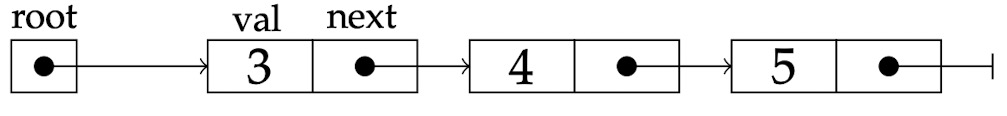
\includegraphics[width=0.5\linewidth]{images/Screenshot 2024-05-30 at 19.03.47.jpg}
    \end{figure}
    \begin{minipage}{0.5\textwidth}
    \item Corresponding declaration in C:
    \begin{lstlisting}
struct node {
    int val;
    struct node* next;
};

struct node* root;
\end{lstlisting}
\end{minipage}
\item Accessing a field: \texttt{p->a}
\end{itemize}
Populating a list with integers:\\

\begin{center}
\begin{minipage}{0.6\textwidth}

\begin{lstlisting}
root = malloc(sizeof(struct node));
root->val = 88;
root->next = malloc(sizeof(struct node));

p = root->next;
p->val = 52;
p->next = malloc(sizeof(struct node));

p = p->next;
p->val = 12;
p->next = NULL;

/* print all elements of a list */
p = root;
while (p != NULL) {
    printf("%d,", p->val);
    p = p->next;
}
printf("\n");
\end{lstlisting}
\end{minipage}
\end{center}

Cost of linked list operations:
\begin{itemize}
    \item Insertion at beginning: $O(1)$
    \item Insert at end: $O(n)$
    \item isEmpty: $O(1)$
    \item Delete: $O(n)$
    \item Print: $O(n)$
\end{itemize}
Previous code fragments for working with the linked list access the list through global variable root => not good
\begin{itemize}
    \item Thus, there can be at most one linked list
    \item The code does not allow us to define and use multiple linked lists
\end{itemize}

Variants of linked lists:
\begin{itemize}
    \item Lists with explicit tail
    \begin{itemize}
        \item Do have an extra pointer to the last item of the list
        \item No need to scan the entire list if an operation applies only to the last item
    \end{itemize}
    \item Doubly linked list
    \begin{itemize}
        \item Each node has a field with a pointer to the previous node of the linked list
        \item Provides means to quickly navigate back and forth in the linked list
    \end{itemize}
\end{itemize}


\subsection{ADT: Abstract Data Types}
